\chapter{SpMV on FPGA METHODOLOGY}
\label{chp:method}

\begin{figure}
    \centering
    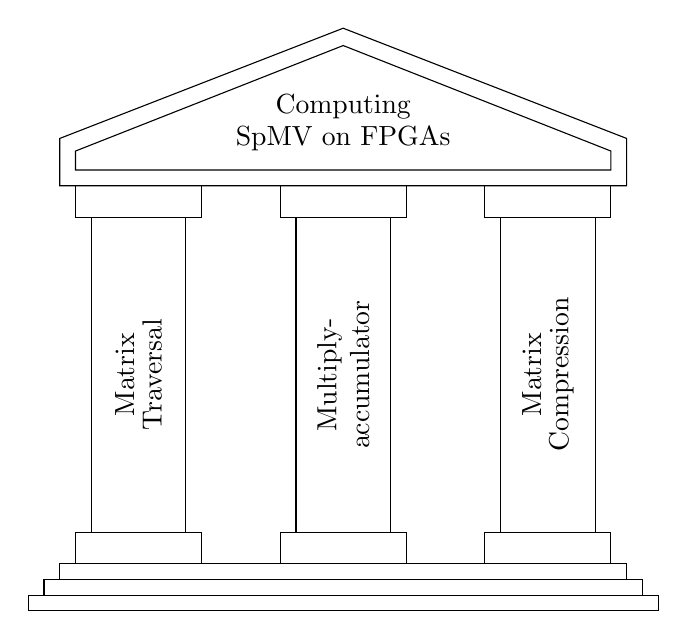
\begin{tikzpicture}[scale=2]
        \draw (0,0) rectangle (4,.1);
        \draw (.1,.1) rectangle (3.9,.2);
        \draw (.2,.2) rectangle (3.8,.3);

        \draw (.3,.3) rectangle (1.1,.5);
        \draw (1.6,.3) rectangle (2.4, .5);
        \draw (2.9, .3) rectangle (3.7, .5);
        \draw (.4,.5) rectangle (1,2.5);
        \node at (.7,1.5) [rotate=90]{\shortstack{Matrix\\Traversal}};

        \draw (1.7,.5) rectangle (2.3,2.5);
        \node at (2,1.5) [rotate=90]{\shortstack{Multiply-\\accumulator}};

        \draw (3,.5) rectangle (3.6,2.5);
        \node at (3.3,1.5) [rotate=90]{\shortstack{Matrix\\Compression}};

        \draw (.3,2.5) rectangle (1.1,2.7);
        \draw (1.6,2.5) rectangle (2.4, 2.7);
        \draw (2.9, 2.5) rectangle (3.7, 2.7);

        \draw (.2,2.7) -- (3.8,2.7) -- (3.8,3) -- (2,3.7) -- (.2,3) -- cycle;
        \draw (.3,2.8) -- (3.7,2.8) -- (3.7, 2.92) -- (2,3.59) -- (.3,2.92) -- cycle;
        \node at (2,3.1) {\shortstack{Computing\\SpMV on FPGAs}};
    \end{tikzpicture}
    \caption[The three pillars of optimization for computing SpMV on FPGAs.]{Because different aspects limit the performance of SpMV on FPGAs, no one optimization will lead to significant benefit for SpMV. We identified these three optimizations that together lead to a significant performance benefit.}
    \label{fig:pillars}
\end{figure}

In the previous chapter, we discussed how others approach computing SpMV on FPGAs and other processors. We build upon these ideas and add our own. Three pillars emerged during the design of the hardware description and software: designing the traversal of the matrix, designing the multiply-accumulator, and designing the matrix compression. \figurename~\ref{fig:pillars} abstractly illustrates our view that all three pillars need to be in place to achieve competetive performance. The next three sections describe these pillars and the interactions between them.

\section{First Pillar: Matrix Traversal}
\par The first pillar, matrix traversal, primarily helps with vector reuse. Column traversal has a major effect on vector reuse. Many papers argue that vector caching is the way to achieve $x$ vector reuse for FPGAs [\cite{prelim:umuroglu, prelim:nagar1}]. We disagree. With the ability to use column traversal in a horizontal subsection of say 1000 rows one can perfectly reuse vector values in this section. This requires the storage of 1000 intermediate y values or 8KB. Compare this to caching. Assume there are 10 non-zero elements per row and assume each vector value gets accessed twice. Then to achieve good caching the cache must support 5000 values or 40KB. This also ignores storing the vector indices of the cached values. So, in this example, storing intermediate values is more than 5 times more space efficient than $x$ vector caching.
\par The second advantage of mixing row and column traversal is that it leads to smaller deltas. In this paper, a delta is the traversal distance between a matrix element and its preceding matrix element in the traversal. To achieve high $x$ vector reuse and small deltas we use row-column-row traversal. Chapter \ref{chp:traversal} discusses matrix traversal in detail.

\section{Second Pillar: Multiply-accumulator}

\par The second pillar, the multiply accumulator, has to accumulate multiple rows at a time to allow different traversals (the first pillar). Several multiply-accumulators exists, but they rely on row-major traversal. Although, we used pre-existing floating-point cores created by Flopoco [\cite{prelim:dedinechin}]. We created an IP core called an Intermediator, which stores intermediate $y$ values and allows for row-column-row traversal. Chapter \ref{chp:mac} discusses the multiply-accumulator in detail.

\section{Third Pillar: Matrix Compression}
\par The third pillar, compression, may be the most important for FPGAs. Compression of the matrix has a large amount of importance, because reading the matrix takes up a majority of the memory bandwidth. The current view in the SpMV field does not count preprocessing of the matrix towards the SpMV runtime. This is because SpMV is usually used in iterative and repetitive methods. We agree with this sentiment. Matrix compression is split into to seperate problems: index compression and floating point compression.
\subsection{Index Compression}
\par Using deltas to compress indices is the first and easiest step towards this pillar. Many compression implementations try to align variable length encoding to 4 bit or other size boundaries. We give little regard to boundaries because we find the added compression to be worth the extra FPGA space the decoder needs. Chapter \ref{chp:compression} discusses delta compression in detail.
%
\subsection{Floating Point Compression}
\par Floating point compression is tricky but has a potential to save large amounts of space and thus memory bandwidth. Values repeat more than one would expect in matrices \cite{prelim:kourtis}. Taking advantage of this repetition is the biggest step towards good compression. \figurename~\ref{fig:uniqueVgflops} in the previous chapter showed how much of an effect this pattern has on the performance of our previous SpMV implementation, $R^3$. Chapter~\ref{chp:fzip} discusses our new floating point compression in detail.

\subsection{Multi-port Shared Memory}
\par Because good value compression requires a significant amount of on-chip memory space, we designed a shared memory IP block. This means instead of using 1 RAM block on each PE to store the 512 most common floating point values, we use one RAM block per PE to create a large shared memory to store the 8,192 most common floating point values. Chapter~\ref{chp:memory} discusses the design of the shared memory IP block.%
%
\begin{figure}
\centering
\begin{tikzpicture}[scale=1]
\draw [dashed](-6,0) -- (4,0);
\node at (.1,-2) {\large \shortstack{External\\Memory}};
\node at (.1,-1) [draw, trapezium, trapezium right angle=70, trapezium left angle=-70,  minimum width=1.5cm, minimum height=1cm, inner xsep=-7pt](x){$x$ Vector};
\node at (-3,-1.25) [draw,trapezium, trapezium right angle=70, trapezium left angle=-70,  minimum width=1.5cm, minimum height=1.5cm, inner xsep=-12pt](a){$A$ Matrix};
\node at (2.5,-1) [draw, trapezium, trapezium right angle=70, trapezium left angle=-70, minimum width=0cm, minimum height=1cm, inner xsep=-7pt](y){$y$ Vector};

\node at (0, 3) {\large $R^3$ Processing Element};
\draw [dashed] (-6,1.5) -- (-3,1.5);
\node at (-4.5, 1.5) [draw, rectangle, minimum height=2cm, minimum width=3cm](dec){};
\node at (-5.3,1.5)[rotate=90, anchor=south,fill=white]{Decoder};
\node at (-4.5,2) {Value};
\node at (-4.5,1) {Index};
\node at (-4.5, 3.5) [color=black](vCache){Shared Memory};
\path [draw, color=black] (vCache.north east) to (vCache.south east) to (vCache.south west) to (vCache.north west);
\node at (1,1.5) [draw, rectangle, minimum height=2.1cm, minimum width=5cm, label={[label distance=-.5cm]90:Multiply-Accumulator}](acc){};
\node at (acc) [draw, rectangle, xshift=1.8cm, yshift=-.2cm, minimum height=1cm](add){Adder};
\node at (acc) [draw, rectangle, xshift=0cm, yshift=-.2cm, minimum height=1cm](int){\shortstack{Inter-\\mediator}};
\node at (acc) [draw, rectangle, xshift=-1.8cm, yshift=-.2cm, minimum height=1cm](mult){\shortstack{Multi-\\plier}};

\path [draw, thick, >=stealth',->, shorten >=2pt](a) to [] node[fill=white, inner sep=1pt, pos=.4]{\shortstack{val+\\row+col}}(dec);
\path [draw, thick, >=stealth',->, shorten >=2pt, label={[above,sloped]{column}}](dec) to [] node[sloped, fill=white, inner sep=1pt]{col} (x);
\path [draw, thick, >=stealth',->, shorten >=2pt](dec.20) to node[sloped, fill=white, inner sep=1pt]{val} (mult);
\path [draw, thick, >=stealth',->, shorten >=2pt](dec.-20) to node[sloped, fill=white, inner sep=1pt]{row} (mult);
\path [draw, thick, >=stealth',->, shorten >=2pt](mult.120) to [bend left = 30] node[sloped, fill=white, inner sep=1pt]{val+row} (int);

\path [draw, thick, >=stealth',->, shorten >=2pt](x) to [] node[sloped, fill=white, inner sep=1pt]{val} (mult);
\path [draw, thick, >=stealth',->, shorten >=2pt](int.north) to [bend left = 20] node[sloped, fill=white, inner sep=1pt]{val+val+row} (add.50);
\path [draw, thick, >=stealth',->, shorten >=2pt](add.-50) to [bend left = 40] node[sloped, fill=white, inner sep=1pt]{val+row} (int);
\path [draw, thick, >=stealth', ->, shorten >= 2pt](int) .. controls (1,0) and (2.1,0) .. node[sloped, fill=white, inner sep=1pt]{val}  (y);
\path [draw, gray, thick, >=stealth', <->, shorten >=2pt] (vCache) -- (dec);

\end{tikzpicture}
\caption[Diagram of a single processing element.]{A single processing element. The arrows show the flow of data through the processing element. Although this diagram shows the memory access to each of the 3 places in memory as separate, they share one memory port. The diagram also does not show the FIFOs that help keep the pipeline full.}
\label{fig:SpMV}
\end{figure}%
%

\begin{figure}
\centering
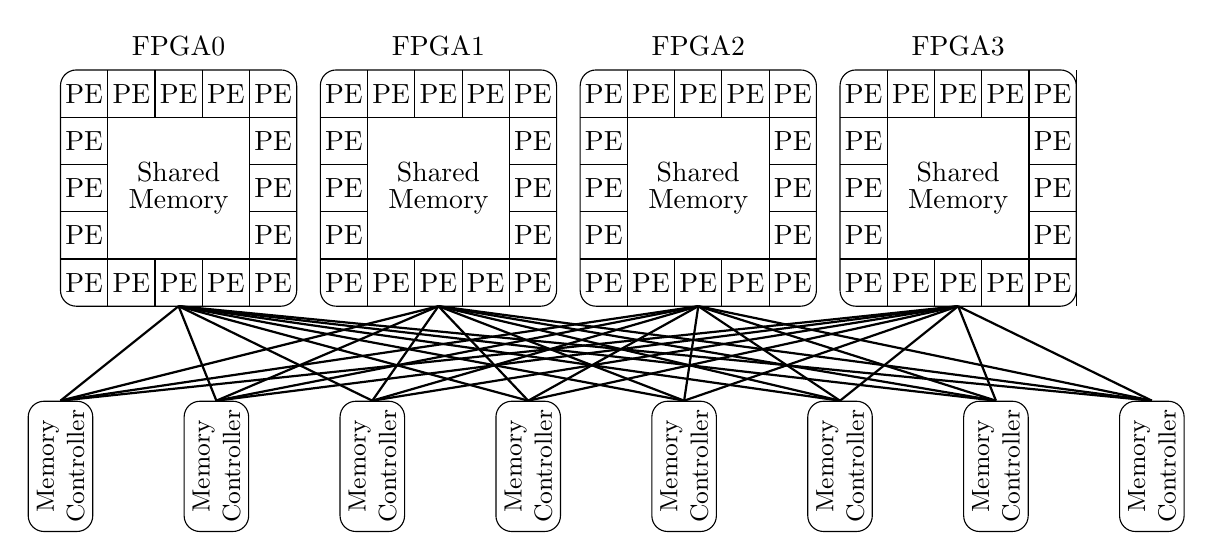
\begin{tikzpicture}[scale=.6]
\node at (3,6){FPGA0};
\node at (8.5,6){FPGA1};
\node at (14,6){FPGA2};
\node at (19.5,6){FPGA3};
\foreach \x in {1,...,4,5,6.5,7.5,...,10.5,12,13,...,16,17.5,18.5,...,21.5}
    \foreach \y in {1,...,5}
    {
        %\draw (\x, \y) +(-.5,-.5) rectangle ++(.5,.5);
        %\draw (\x, \y) node{\shortstack{$R^3$\\PE}};
        \draw (\x, \y) node{\shortstack{PE}};
    }
\foreach \x in {1.5,2.5,3.5,4.5,7,8,9,10,12.5,13.5,14.5,15.5,18,19,20,21,22}
{
    \path[draw] (\x, .5) -- (\x, 5.5);
}
\foreach \x in {.5,6,11.5,17}
{
    \foreach \y in {1.5,2.5,3.5,4.5}
    \path[draw] (\x, \y) -- (\x+5, \y);
}
\draw (.5,.5) [rounded corners=.2cm]rectangle (5.5,5.5);
\draw (6,.5) [rounded corners=.2cm]rectangle (11,5.5);
\draw (11.5,.5) [rounded corners=.2cm]rectangle (16.5,5.5);
\draw (17,.5) [rounded corners=.2cm]rectangle (22,5.5);
\foreach \x in {3,8.5,14,19.5}{
    \node at (\x, 3)[draw, fill=white, minimum width=1.8cm, minimum height=1.8cm,inner sep=0,outer sep=0]{\shortstack{Shared\\Memory}};
}
\foreach [count=\i] \x in {.5,3.8,7.1,...,25} %0,3.3,6.6,...,24}
{
    \FPeval{\minus}{round(\i-1,0)};
    %\draw (\x, -2) +(-.6,-.5) [rounded corners=.2cm] rectangle ++(1.2, .5);
    \small
    \draw (\x, -1.5) node[draw, rectangle,rounded corners=.2cm,rotate=90,anchor=east]{\shortstack{Memory \\Controller~\minus}};
    \normalsize
    %\draw (\x, -2) +(.3, 0) node{\shortstack{MC\i}};
}
\foreach \ae in {3, 8.5, 14, 19.5}
{
    \foreach \mc in {.5,3.8,7.1,...,25}
    {
        \draw[thick] (\ae, .5) -- (\mc, -1.5);
    }
}
%\path[draw, dashed] (.5,-.5) -- (18,-.5);
%\node at (9.25,-.5) [rectangle,fill=white,inner sep=2pt](a){40GB/s Sustained Memory Bandwidth};

\end{tikzpicture}
\caption[Modified high-level diagram of the Convey HC-2ex.]{Our implementation has one shared memory for storing repeating values in the sparse matrices.}
\label{fig:highlevel2}
\end{figure}
\section{High Level Design}
Designing high performance reconfigurable computing implementations has a general two step process, which we follow. First, design one processing element (PE) to solve the problem (see \figurename~\ref{fig:SpMV}). Second, replicate that PE until all the FPGAs are full (see \figurename~\ref{fig:highlevel2}). In addition to the PEs, we have a shared memory on the FPGA as well.

The PEs recieve instructions through a 1D systolic array. Each PE has 14 registers. Each PE has 8 instructions: RESET, READ\_REGISTER, WRITE\_REGISTER, WRITE\_DELTA\_CODES, WRITE\_FZIP\_CODES, WRITE\_SHARED\_MEMORY, and COMPUTE\_SPMV.

The PE themselves have 2 major components. First, the decoder block that requests the compressed matrix data and decodes it into row and column indices and floating point values. Second, the multiply-accumulator, where the actual SpMV computation takes place.

To Parallelize the SpMV computation we split the problem into $N$ smaller SpMV computations each given to one processing element. In hardware we connect each processing element to an external memory port and a shared memory port. Chapter \ref{chp:memory} discusses the high level design in detail.
%\par We separate our contributions into 5 pieces, the next 5 chapters. Chapter~\ref{chp:mac} focuses entirely on the first pillar, the multiply accumulator design. Chapter~\ref{chp:compression} focuses on pillars 2 and 3 with discussing matrix traversal and compressing indices with delta compression. Chapter~\ref{chp:fzip} focuses on the second part of pillar 3, value compression. We found good value compression requires a large amount of on-chip memory, therefore, Chapter~\ref{chp:memory} focuses on the design of a large memory shared by multiple processing elements.
